\documentclass[crop=true]{standalone}

% tikz
\usepackage{tikzscale}
\usepackage{pgfplots}
\usepackage{mathtools}
\pgfplotsset{compat=1.18}
% \usepgfplotslibrary{external}
% \tikzexternalize[prefix=./]
% \newcommand{\includetikz}[1]{%
%     \tikzsetnextfilename{#1}%
%     \input{#1.tikz}%
% }
% explicitly set line width to avoid different widths in different pdf viewers
\tikzset{every picture/.style={line width=0.5pt}}
% groupplots
\usepgfplotslibrary{groupplots}
\usetikzlibrary{pgfplots.groupplots}
\usetikzlibrary{matrix}
\usetikzlibrary{patterns}

\begin{document}
%
% HOWTO: Convert a Matlab figure to svg via tikz
%
% 1. Create and save Matlab figure      								savefig('<figure-path>/<figure-name>.fig')
% 2. Convert fig to tikz:										        convertToTikz('<figure-path>/<figure-name>.fig')
% 3. Update <figure-path>/<figure-name> in the \input command below
% 4. Create dvi of figure:										        pdflatex -output-format=dvi main
% 5. Convert dvi to svg:										        dvisvgm main.dvi --font-format=woff --optimize -o ./figures/dynamics-systems/feedback_neuralNetContrSys.svg
% 6. Add to website         										    <img src="<figure-path>/<figure-name>.svg"/>
%
% \input{./<figure-path>/<figure-name>.tikz}
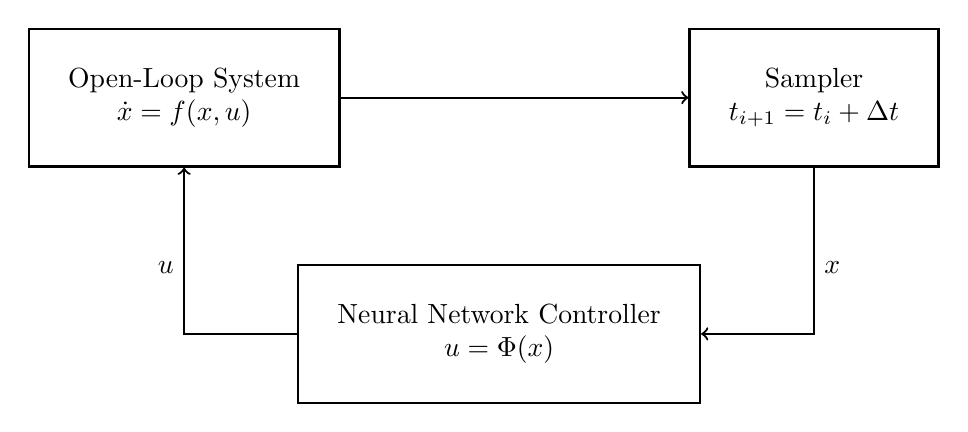
\begin{tikzpicture}
    [
    arrow/.style={
        thick,
        ->
    },
    box/.style={
        draw,
        rectangle,
        thick,
        inner sep=0.5cm,
        align=center % align is required for multi-line text
    },
    ]

    \draw (0,0) node[box] (sys) {Open-Loop System \\ $\dot{x}=f(x,u)$};
    \draw (8,0) node[box] (sampler) {Sampler \\ $t_{i+1} = t_{i} + \Delta t$};
    \draw (4,-3) node[box] (nn) {Neural Network Controller \\ $u = \Phi(x)$ };

    \draw [arrow] (sys) -- (sampler);
    \draw [arrow] (sampler) |- (nn) node[pos=.3,anchor=west] {$x$};
    \draw [arrow] (nn) -| (sys) node[pos=.7,anchor=east] {$u$};


\end{tikzpicture}
%
% Note: Make sure that there are no empty lines within the document environment for standalone to properly crop the image.
%
\end{document}